% Options for packages loaded elsewhere
\PassOptionsToPackage{unicode}{hyperref}
\PassOptionsToPackage{hyphens}{url}
\PassOptionsToPackage{dvipsnames,svgnames,x11names}{xcolor}
%
\documentclass[
  authoryear,
  preprint]{elsarticle}

\usepackage{amsmath,amssymb}
\usepackage{iftex}
\ifPDFTeX
  \usepackage[T1]{fontenc}
  \usepackage[utf8]{inputenc}
  \usepackage{textcomp} % provide euro and other symbols
\else % if luatex or xetex
  \usepackage{unicode-math}
  \defaultfontfeatures{Scale=MatchLowercase}
  \defaultfontfeatures[\rmfamily]{Ligatures=TeX,Scale=1}
\fi
\usepackage{lmodern}
\ifPDFTeX\else  
    % xetex/luatex font selection
\fi
% Use upquote if available, for straight quotes in verbatim environments
\IfFileExists{upquote.sty}{\usepackage{upquote}}{}
\IfFileExists{microtype.sty}{% use microtype if available
  \usepackage[]{microtype}
  \UseMicrotypeSet[protrusion]{basicmath} % disable protrusion for tt fonts
}{}
\makeatletter
\@ifundefined{KOMAClassName}{% if non-KOMA class
  \IfFileExists{parskip.sty}{%
    \usepackage{parskip}
  }{% else
    \setlength{\parindent}{0pt}
    \setlength{\parskip}{6pt plus 2pt minus 1pt}}
}{% if KOMA class
  \KOMAoptions{parskip=half}}
\makeatother
\usepackage{xcolor}
\setlength{\emergencystretch}{3em} % prevent overfull lines
\setcounter{secnumdepth}{5}
% Make \paragraph and \subparagraph free-standing
\makeatletter
\ifx\paragraph\undefined\else
  \let\oldparagraph\paragraph
  \renewcommand{\paragraph}{
    \@ifstar
      \xxxParagraphStar
      \xxxParagraphNoStar
  }
  \newcommand{\xxxParagraphStar}[1]{\oldparagraph*{#1}\mbox{}}
  \newcommand{\xxxParagraphNoStar}[1]{\oldparagraph{#1}\mbox{}}
\fi
\ifx\subparagraph\undefined\else
  \let\oldsubparagraph\subparagraph
  \renewcommand{\subparagraph}{
    \@ifstar
      \xxxSubParagraphStar
      \xxxSubParagraphNoStar
  }
  \newcommand{\xxxSubParagraphStar}[1]{\oldsubparagraph*{#1}\mbox{}}
  \newcommand{\xxxSubParagraphNoStar}[1]{\oldsubparagraph{#1}\mbox{}}
\fi
\makeatother


\providecommand{\tightlist}{%
  \setlength{\itemsep}{0pt}\setlength{\parskip}{0pt}}\usepackage{longtable,booktabs,array}
\usepackage{calc} % for calculating minipage widths
% Correct order of tables after \paragraph or \subparagraph
\usepackage{etoolbox}
\makeatletter
\patchcmd\longtable{\par}{\if@noskipsec\mbox{}\fi\par}{}{}
\makeatother
% Allow footnotes in longtable head/foot
\IfFileExists{footnotehyper.sty}{\usepackage{footnotehyper}}{\usepackage{footnote}}
\makesavenoteenv{longtable}
\usepackage{graphicx}
\makeatletter
\newsavebox\pandoc@box
\newcommand*\pandocbounded[1]{% scales image to fit in text height/width
  \sbox\pandoc@box{#1}%
  \Gscale@div\@tempa{\textheight}{\dimexpr\ht\pandoc@box+\dp\pandoc@box\relax}%
  \Gscale@div\@tempb{\linewidth}{\wd\pandoc@box}%
  \ifdim\@tempb\p@<\@tempa\p@\let\@tempa\@tempb\fi% select the smaller of both
  \ifdim\@tempa\p@<\p@\scalebox{\@tempa}{\usebox\pandoc@box}%
  \else\usebox{\pandoc@box}%
  \fi%
}
% Set default figure placement to htbp
\def\fps@figure{htbp}
\makeatother

\usepackage{booktabs}
\usepackage{caption}
\usepackage{longtable}
\usepackage{colortbl}
\usepackage{array}
\usepackage{anyfontsize}
\usepackage{multirow}
\makeatletter
\@ifpackageloaded{caption}{}{\usepackage{caption}}
\AtBeginDocument{%
\ifdefined\contentsname
  \renewcommand*\contentsname{Table of contents}
\else
  \newcommand\contentsname{Table of contents}
\fi
\ifdefined\listfigurename
  \renewcommand*\listfigurename{List of Figures}
\else
  \newcommand\listfigurename{List of Figures}
\fi
\ifdefined\listtablename
  \renewcommand*\listtablename{List of Tables}
\else
  \newcommand\listtablename{List of Tables}
\fi
\ifdefined\figurename
  \renewcommand*\figurename{Figure}
\else
  \newcommand\figurename{Figure}
\fi
\ifdefined\tablename
  \renewcommand*\tablename{Table}
\else
  \newcommand\tablename{Table}
\fi
}
\@ifpackageloaded{float}{}{\usepackage{float}}
\floatstyle{ruled}
\@ifundefined{c@chapter}{\newfloat{codelisting}{h}{lop}}{\newfloat{codelisting}{h}{lop}[chapter]}
\floatname{codelisting}{Listing}
\newcommand*\listoflistings{\listof{codelisting}{List of Listings}}
\makeatother
\makeatletter
\makeatother
\makeatletter
\@ifpackageloaded{caption}{}{\usepackage{caption}}
\@ifpackageloaded{subcaption}{}{\usepackage{subcaption}}
\makeatother
\journal{Open Quaternary}

\usepackage[]{natbib}
\bibliographystyle{elsarticle-harv}
\usepackage{bookmark}

\IfFileExists{xurl.sty}{\usepackage{xurl}}{} % add URL line breaks if available
\urlstyle{same} % disable monospaced font for URLs
\hypersetup{
  pdftitle={Biogeography of crop progenitors and wild plant resources in the terminal Pleistocene and Early Holocene of West Asia, 14.7--8.3 ka},
  pdfauthor={Joe Roe; Amaia Arranz-Otaegui},
  colorlinks=true,
  linkcolor={blue},
  filecolor={Maroon},
  citecolor={Blue},
  urlcolor={Blue},
  pdfcreator={LaTeX via pandoc}}


\setlength{\parindent}{6pt}
\begin{document}

\begin{frontmatter}
\title{Biogeography of crop progenitors and wild plant resources in the
terminal Pleistocene and Early Holocene of West Asia, 14.7--8.3 ka}
\author[1,2]{Joe Roe%
\corref{cor1}%
}
 \ead{joeroe@hey.com} 
\author[3]{Amaia Arranz-Otaegui%
%
}


\affiliation[1]{organization={University of
Bern},country={Switzerland},countrysep={,},postcodesep={}}
\affiliation[2]{organization={University of
Copenhagen},country={Denmark},countrysep={,},postcodesep={}}
\affiliation[3]{organization={University of the Basque
Country},country={Spain},countrysep={,},postcodesep={}}

\cortext[cor1]{Corresponding author}


        
\begin{abstract}
This paper presents the first continuous, spatially-explicit
reconstructions of the palaeodistributions of 82 plant species found
regularly in association with early agricultural archaeological sites in
West Asia, including the progenitors of the first crops. We used machine
learning to train an ecological niche model of each species based on its
present-day distribution in relation to climate and environmental
variables. Predictions of the potential ranges of these species at key
stages of the Pleistocene--Holocene transition could then be derived
from these models using downsampled data from palaeoclimate simulations.

The models predict significant reductions and/or shifts in species
ranges in the terminal Pleistocene and Early Holocene compared to
present conditions. Many species that are found throughout the region's
`hilly flanks' today are indicated to have much more restricted
distributions centered on the Levant, Cyprus and Western Anatolia. In
addition, overall ranges shrunk by an average of c.~25\% from the
terminal Pleistocene to the Early Holocene. The models performance in
predicting the occurrence of specific species at archaeological sites is
highly variable, but in aggregate the predictions are coherent and align
with broad-scale trends in the ubiquity and relative abundance of
species in the archaeological record.
\end{abstract}





\end{frontmatter}
    

\section{Introduction}\label{introduction}

The Pleistocene--Holocene transition in West Asia marked a turning point
in global environmental history, as humans brought the first plants
under cultivation and began modifying surrounding ecosystems to support
their own subsistence. West Asia is part of the native range of a
remarkable number of domesticable plant species, including wild
relatives of wheat, barley, peas, lentils, and other crops of global
importance \citep{HarlanZohary1966, Diamond2002, ZoharyEtAl2012}. These
species supported uniquely dense and complex Late Epipalaeolithic
(15--11.7 ka) societies \citep{BarYosef1998, MaherEtAl2012} based on
foraging \citep{HarrisHillman1989, Colledge2001, WeissEtAl2004} and
eventually plant management and pre-domestication cultivation
\citep{Colledge2001, WeissEtAl2006, Harris2007, WillcoxEtAl2008}. The
first agro-ecosystems emerged as these plants were domesticated in the
Pre-Pottery Neolithic period (11.7--8.5 ka) and were shaped by the
broader ecosystem in which it was embedded.

Decades of research in archaeobotany and zooarchaeology have
reconstructed the subsistence economies of Late Epipalaeolithic and
Neolithic sites in great detail. Together with studies of other
environmental archaeological records and a variety of palaeoclimate
archives \citep{JonesEtAl2019}, they also tell us much about the
environments surrounding these settlements. However, each of these
sources of evidence is subject to the wide variety of taphonomic and
recovery biases that are inherent in any direct record of the past. They
are also, by definition, records of the (human) environment at
particular times and places. Interpolating these snapshots to give a
holistic picture of the regional ecologies is not straightforward -- to
date, it has tended to rely on non-explicit, inductive modelling. The
majority are also filtered through human action, producing a mixed
single that makes it difficult to disentangle anthropic effects from the
background of environmental change in this period of rapid climatic
alteration.

In this paper we present a complementary, deductive approach based on
ecological niche modelling. Rather than inferring environmental
conditions from preserved physical evidence, we predict the ranges of
individual species relevant to human subsistence based on a model of
their current environmental niche and simulations of past palaeoclimate.
Though hypothetical, this gives us an independent line of evidence on
past ecologies that is independent of the environmental archaeological
and palaeoclimatic records. This means that the ancient data can be
reserved for assessing the model's ability to `hindcast' past
conditions. In this sense, discrepencies between the two records are
perhaps the most interesting result, as they indicate processes
affecting one or both records that are not fully accounted for and
therefore generate new questions. Our computational approach is also
readily scaled up, allowing us to model spatially-explicit
palaeodistributions for a large number of species, for the whole region,
under multiple past climatologies.

\section{Background}\label{sec-bg}

The transition to agriculture represents one of the most fundamental
changes in human history. West Asia is one of the regions where this
process has been studied in the most detail: decades of research have
traced the gradual development of a Neolithic way of life and the
changes that occurred in the plant species and their geographical
distribution as a result. Although archaeobotanical assemblages can be
biased due to issues of preservation, sampling, recovery techniques, and
lab procedures \citep{Dennel1976, HastorfPopper1988}---and although they
include not just food remains but plant resources that were used for
other purposes or arrived at the site accidentally
\citep{HastorfPopper1988}---large-scale studies have still revealed
coherent patterns in the exploitation of plants over time
\citep{ColledgeEtAl2004, ArranzOtaeguiEtAl2016}.

The possibility of an abrupt, geographically-constrained process of
plant domestication was proposed in the 1990s
\citep{HillmanDavies1990, HillmanDavies1992, HeunEtAl1997, OzkanEtAl2002}
and developed as an explanatory model in the 2000s
\citep{LevYadunEtAl2000, GopherEtAl2001, AbboEtAl2005}. As part of this
model, some authors
\citep{LevYadunEtAl2000, GopherEtAl2001, AbboEtAl2010, AbboEtAl2012}
argued that eight plant species, collectively referred to as `founder
crops' or the `Neolithic crop package' \citep{ZoharyHopf1988} were
selected and domesticated once, without any phase of pre-domestication
cultivation \citep[p.~177]{AbboEtAl2011}. This process could have been
rapid under strong artificial selection
\citep{HillmanDavies1990, HillmanDavies1992} and may have occurred in a
single region or `core area' -- generally located in southeast Turkey
\citep{LadizinskyAdler1976, HeunEtAl1997, OzkanEtAl2002, OzkanEtAl2005, MoriEtAl2003, LuoEtAl2007}.
From this single point of origin, it was supposed that domesticated or
semi-domesticated plants radiated outwards to other regions
\citep{AbboEtAl2006, KilianEtAl2007, OzkanEtAl2011}.

The `short gestation' paradigm was challenged by others
\citep{Helbaek1969, Harris1989, Kislev1989, Colledge2001, WeissEtAl2004, WillcoxEtAl2008, FullerEtAl2018}.
Helbæk \citep[in][]{Kirkbride1966} argued that before the appearance of
domesticated plants, a phase of cultivation of wild seeds must have
taken place. The existence of a phase of cultivation of morphologically
wild cereals or `pre-domestication cultivation' was identified in the
archaeological record through the study of plant domestication traits
such as grain size, shattering v. non-shattering rachises. The
archaeobotanical evidence shows that during the Pre-Pottery Neolithic A
(PPNA) cereals exhibited sizes similar to those recorded in domestic
species, but their dispersal mechanism was still the same as the one
present in morphologically-wild species \citep[i.e.~shattering,
see][]{Kirkbride1966, Kislev1989, HillmanEtAl2001, Colledge2001, WillcoxEtAl2008}.
This evidence suggested that wild cereal stands could have been
cultivated for as much as a thousand years before non-shattering
domestic forms became prevalent in the archaeological record
\citep{TannoWillcox2006, TannoWillcox2012, ArranzOtaeguiEtAl2016}.
Additional archaeobotanical
\citep{Colledge2001, WillcoxEtAl2008, WillcoxEtAl2009, RiehlEtAl2013, ArranzOtaeguiEtAl2016, WeideEtAl2018, DoucheWillcox2018, WhitlamEtAl2018}
and genetic data
\citep{BadrEtAl2000, MolinaCanoEtAl2005, KilianEtAl2007, OzkanEtAl2011, IobBotigue2023}
in recent years has further challenged the short-gestation model to
explain the origins of plant domestication and agriculture in West Asia.

Similarly, the concept of a limited set of eight `founder crops'
\citep{ZoharyHopf1988} that were the first species cultivated,
domesticated and then spread as the basis of Neolithic agricultural
systems, is not supported by the latest evidence. Our previous analyses
of the composition of available archaeobotanical datasets shows that
these crops were of marginal importance during the Epipalaeolithic
period \citep{ArranzOtaeguiEtAl2018} and that Neolithic subsistence did
not rely either solely or primarily on the exploitation of these species
\citep{ArranzOtaeguiRoe2023}. Instead, multiple species of grasses,
legumes, fruits, nuts, and other plants were exploited over the Late
Pleistocene-Early Holocene transition in southwest Asia.

\subsection{Biogeography and agricultural
origins}\label{biogeography-and-agricultural-origins}

The study of the natural distribution of the progenitors of domesticated
crops has been a central part of discussions on the origins of
agriculture and plant domestication from the beginning.
\citet{Humboldt1807} acknowledged the importance of the natural
distribution of wild species to explain the origin and domestication of
crops like spelt and rye. \citet{Candolle1886} integrated the study of
plant ecology and biogeography and influenced \citet{Darwin1859}, who
later reflected in detail about the geographical distribution of plants
and species diversity. At that time, there was intense debate about
whether there were single or multiple ``centres of creation'' of
species. Researchers aimed to evaluate whether plant and animal species
emerged in the same locations where they were currently distributed.

After Darwin, this early interest in crop origins evolved into more
specific discussions about the ``centres of plant domestication''.
\citet{Vavilov1926} was among the first to seek to determine the number
of regions in which plants had been independently domesticated
\citep{Harris1990}. His main method was `differential phytogeography':
he classified the variation within a crop and established the regions of
maximum diversity, to locate the geographic regions in which crops
originated. Using this method, Vavilov suggested that there were at
least eight centres of origin. His work was later criticised by
\citet{Harlan1971}, who argued that `centres of origin' and `centres of
diversity' had to be separated. For Harlan, a `centre' was as an ``area
in which things originate and out of which things are dispersed''
\citep[p.~468]{Harlan1971}, and he suggested that three main centres of
origin of domesticated crops existed. He further indicated that
Vavilov's approach to the question was simplistic and that more data
proxies had to be considered (e.g.~archaeology, history, geology), an
approach more in the tradition of \citet{Candolle1886}. Indeed, the
inclusion of archaeobotany and genetics in the last decades, together
with the study of wild relative distributions has been fundamental in
characterising the origins of agriculture \citep{FullerColledge2008}. As
a result of modern interdisciplinary studies, the number of recognised
centres of plant domestication has increased considerably, from the
three centres suggested by Harlan in 1971 to the six to eight centres
argued for in the 1990s \citep{Smith1995} and up to as much as 24
potential centres reported in 2009
\citetext{\citealp{PuruggananFuller2009}; \citealp[see
also][]{Fuller2010}}.

Biogeographic research into the centres of origin and/or domestication
of crops has also long informed broader understanding of the process of
agricultural origins. In \emph{Man Makes Himself}, \citet{Childe1936}
correctly located the centre of origin of European agriculture in the
`Fertile Crescent' of West Asia (unlike for example \citet{Pumpelly1908}
before him). This was not based on the region's prehistoric
archaeological record, which at the time had only been cursorily
explored. Instead he was guided to the region by biogeographic work by
Vavilov and \citet{PeakeFleure1927}; only later was this prediction
validated by archaeological work on the Epipalaeolithic and Neolithic of
Palestine \citep{Boyd2018}. In subsequent decades, the search for more
precise origin zones of specific domestic plants relied on the
assumption that ``the locus of domestication of a wild plant would
presumably be within its area of original distribution in the wild
state''
\citetext{\citealp{Butzer1971}; \citealp[paraphrasing][]{Helbaek1959}}
-- and that this ``natural habitat'' has not changed significantly over
the last 12,000 years \citep{Butzer1971}.

Contemporary research on crop origins was pioneered by Harlan and
Zohary, who compared the current distribution of the wild progenitors of
domesticated plants in southwest Asia
\citep{HarlanZohary1966, Zohary1969, Zohary1973, ZoharyHopf1973} to the
rapidly-expanding archaeobotanical record
\citetext{\citealp{Harlan1971}; \citealp{Harlan1977}; \citealp[see
also][]{ZoharyHopf1988}; \citealp{HarlanZohary1966}}. They both were
interested in evaluating which were the wild ancestors of domesticated
crops and studying their natural distribution to understand their
domestication process
\citep{Zohary1969, Zohary1973, ZoharySpiegelRoy1975}. Indeed, the
natural distribution of the wild relatives of domestic plant species was
later used as a criterion to infer `pre-domestic cultivation' in the
archaeological record. For example, the presence of seeds of chickpea at
Jericho led \citet{Hopf1986} to interpret the remains as cultivars, as
the natural distribution of the wild form of chickpea was located
further to the north. The same rationale was applied to the einkorn
remains found at several Pre-Pottery Neolithic sites in the southern
Levant \citep{Hopf1969, Colledge2001}, as the wild progenitors of this
species was thought to be restricted to the northern Levantine area
\citep{HeunEtAl1997, ZoharyEtAl2012}. The same idea---presence of plants
outside their natural range---has been repeated in the literature more
recently by several other authors
\citep{TannoWillcox2006, WillcoxEtAl2008, HillmanEtAl2001}.

Despite the importance of biogeography in the development and validation
of hypotheses regarding the origins of agriculture, there have been few
studies of the wild range of specific crop progenitors or other relevant
plant species \citep[cf.~for domestic animals, e.g.][]{YeomansEtAl2017}.
Observations regarding translocation or range expansion must therefore
rely on a relatively rough and ahistoric notion of a species' `natural
distribution' -- that is, one based primarily on contemporary or
recent-historic occurrences. Yet we know there has been considerable
climatic and environmental change in West Asia since the terminal
Pleistocene \citep{JonesEtAl2019}, so it is very unlikely that these
ranges were in fact static. Reconstructions of broader environments have
attempted to trace their fluctuations through time, either for the
entire region
\citetext{\citealp[e.g.][]{VanZeistBottema1991}; \citealp[Hillman
in][]{MooreEtAl2000}} or parts of it \citep[e.g.][]{Cordova2007}, but
these are at the level of the vegetation zone rather than individual
species. They also invariably rely on what might be called `expert
interpolation' (where the author composes a map based on his or her own
knowledge of the relevant data) rather than an explicit modelling
process. This makes it difficult, if not impossible, for users of such
reconstructions to understand exactly how they were derived or what
could explain, for example, the significant discrepencies between the
predictions of different experts.

\subsection{Ecological niche modelling in
archaeology}\label{ecological-niche-modelling-in-archaeology}

Ecological niche modelling or species distribution modelling is widely
used by ecologists to predict the geographic range of a species based on
a set of environmental predictors \citep{FranklinMiller2009}.
Essentially, it involves combining records of where an organism has been
observed with environmental data (climate, topography, etc.) for those
locations to model the range of environmental values at which that
species -- its environmental niche. This model can then be used to
predict the range of the organism in question either in the same or a
different environment. \citet{TownsendPetersonSoberon2012} suggests
reserving the term `species distribution modelling' for when the method
is used to recover the verifiable range of a species in a real and
existing environment, and using `ecological niche modelling' as the
broader term covering hypothetical or predictive applications -- a
convention we follow here when referring to predictive or `hindcast'
models of past ranges. Within this overarching framework, ecological
niche modelling encompasses a wide range of applications and a variety
of potential environmental predictors, modelling approaches, and
methodologies, which we will not attempt to review here.

Ecological niche modelling has long been of interest to archaeologists
as both a means of exploring the biological niche of humans and for
reconstructing the past environments they inhabited
\citep{DavidPollyEronen2011, FranklinEtAl2015}. In the first sense, it
has been used most extensively to model the range of humans and other
hominin species
\citep[e.g.][]{BenitoEtAl2017, YousefiEtAl2020, BanksEtAl2021, YaworskyEtAl2024a, YaworskyEtAl2024b, GuranEtAl2024},
especially in the Palaeolithic. This overlaps with what archaeologists
usually call generically `predictive modelling'
\citep{VerhagenWhitley2020}---or more precisely `site distribution
modelling'---which is essentially the same approach as (and often
borrows methodologies from) ecological niche modelling but applied to
the occurrence of archaeological sites. Here what is modelled is not
strictly a biological niche alone, but also aspects of human geography,
taphonomy, and archaeological visibility. These applications can be
distinguished from `palaeoecological niche modelling', where the object
of model remains, as in ecology, a non-human biological niche.

\citet{FranklinEtAl2015} review palaeoecological niche modelling and
advocate for its greater adoption in environmental archaeology. In an
early application to West Asia, \citet{ConollyEtAl2012} used the
occurrence of wild and domestic \emph{Bos} remains at prehistoric
archaeological sites to map the evolving niche of cattle over the
Pleistocene--Holocene transition. It has been used to model the
availability of fauna exploited by humans at wider scales
\citep[e.g.][]{deAndresHerreroEtAl2018, YaworskyEtAl2023} and, in a West
Asian context, of foraged plant resources in the landscape around the
Neolithic sites on the Konya Plain \citep{CollinsEtAl2018}. Modelling
the spread of crops has been another significant archaeological
application \citep[e.g.][]{KrzyzanskaEtAl2022, Krzyzanska2023}, though
not as yet applied to West Asia.

In the majority of studies to date (palaeo)ecological niche modelling
has been applied to archaeological data in an `inductive' fashion,
i.e.~faunal and botanical remains from ancient sites are used as the
occurrence dataset for training a model using either past or present
environmental data. However, both the zooarchaeological and
archaeobotanical records are sparse and subject to a complex array of
depositional, taphonomic and recovery biases factors that , many of
which are not fully understood and/or cannot be corrected for. This
means that while the archaeological attestation of the presence of a
species might generally be relied upon, it is highly unlikely that its
absence is representative of true past distributions.

The alternative approach is to train the model using contemporary
occurrence and environmental data and then use palaeoenvironmental data
to `hindcast' its predictions backwards in time. Like
\citet{FranklinEtAl2015}, we view the hindcasting approach as more
promising, because training datasets for both occurrences and
environment are far more readily available, complete and reliable for
the present than the past. There is some scepticism in the ecological
niche modelling literature about the ability of such models to make
accurate predictions in unknown environments \citep[like the
past,][]{FranklinEtAl2015}, but here the hindcasting approach also
presents an opportunity: it reserves archaeological occurrence data as
an independent dataset that can be used to assess the retrodictive
performance of the model. This possibily was suggested by
\citet{FranklinEtAl2015} but to our knowledge our study represents the
first attempt to actually do so.

The major practical limitation of the hindcasting approach is that it
relies on spatially explicit, high resolution palaeoenvironmental
surfaces with continuous coverage of the region and periods of interest.
Until recently, this has not been widely available for most
applications, which is perhaps why only a minority of studies use it
\citep[cf.][]{KrzyzanskaEtAl2022, YaworskyEtAl2023}. In this study, we
are able to take advantage of the increasing availability of high
resolution, global palaeoclimate data derived from simulation
experiments with general circulation models of climate
\citep{BrownEtAl2018, BrownEtAl2020, KargerEtAl2023}.

\section{Data and model}\label{data-and-model}

\begin{figure}

\centering{

\pandocbounded{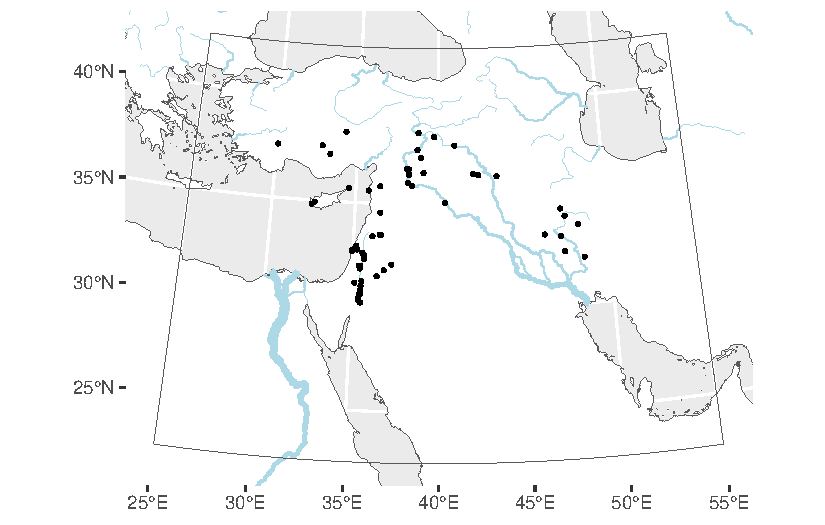
\includegraphics[keepaspectratio]{paper_files/figure-pdf/fig-region-1.pdf}}

}

\caption{\label{fig-region}Late Epipalaeolithic \& Pre-Pottery Neolithic
archaeological sites used to generate modelled flora}

\end{figure}%

The aim of our study was to model the biogeography of species relevant
to human subsistence economies in West Asia (excluding the Southern
Arabian peninsula, see Figure~\ref{fig-region}) during the
archaeological Late Epipalaeolithic (15--11.7 ka) and Pre-Pottery
Neolithic (11.7--8.3 ka) periods. Based on current understandings, we
assume that plant-based subsistence during this period was broad,
geographically- and temporally-varied, and reflects a gradual,
geographically decentred, and nonlinear tranistion to greater reliance
on cultivars (i.e.~agriculture, see Section~\ref{sec-bg}). Our starting
point was a list of 66 taxa (Table~\ref{tbl-results-summary}) comprising
the identified species observed at at least 3 Late
Epipalaeolithic/Pre-Pottery Neolithic sites, according to our previous
study of the regional archaeobotanical data
\citep{ArranzOtaeguiRoe2023}. This was based on dataset collated from
three previously published regional archaeobotanical databases: ADEMNES
\citep{ADEMNES}, ORIGINS \citep{ORIGINS}, and COMPAG
\citetext{\citealp{LucasFuller2018}; \citealp{FullerEtAl2018}; \citealp[based
on][]{ColledgeEtAl2004}; \citealp{ShennanConolly2007}}. We did not
attempt to distinguish between the source of the remains
\citep[cf.][]{WallaceEtAl2018}; archaeobotanical assemblages are subject
to a variety of preservational and recovery biases, so by no means were
all the species on our list consumed or even deliberately collected by
people. However, we assume that there presence at a site of human
settlement at least implies that they were part of the wider ecosystem
that supported habitation there.

The taxonomic identifications of archaeobotanical material given in our
source databases were previously controlled to ensure consistency
between sources and to remove taxa that cannot be reliably distinguished
\citep[for details see][]{ArranzOtaeguiRoe2023}. Taxonomic names were
then matched to the canonical form specified in the GBIF Backbone
Taxonomy \citep{GBIFSecretariat2023} so they could be related to modern
occurrences. Archaeologically-attested domestic species meeting our
inclusion criteria were substituted for their wild progenitors (where
different) when gathering occurrence data, since the domestic forms are
now widespread and presumably uninformative of the species original
niche.

\subsection{Occurrence data}\label{sec-occ-data}

\begin{verbatim}
Rows: 1 Columns: 11
-- Column specification --------------------------------------------------------
Delimiter: ","
chr  (5): key, doi, license, status, downloadLink
dbl  (3): size, totalRecords, numberDatasets
dttm (3): created, modified, eraseAfter

i Use `spec()` to retrieve the full column specification for this data.
i Specify the column types or set `show_col_types = FALSE` to quiet this message.
\end{verbatim}

Georeferenced occurrence data for West Eurasia between 0 and 60° of
latitude was obtained from the Global Biodiversity Information Facility
(GBIF) using via and the R package `rgbif'
\citep{ChamberlainBoettiger2017, rgbif}. The GBIF dataset
\citep{GBIFDerivedData} excluded fossil occurrences, recorded absences,
and records with missing or dubious coordinates. Although niche models
have reasonable predictive power even with small training samples
\citep{StockwellPeterson2002, HernandezEtAl2006, WiszEtAl2008}, we did
not attempt to model 3 taxa with less than 40 usable occurrences,
following recommendations for niche models generally and Random
Forest-based models specifically
\citep{StockwellPeterson2002, LuanEtAl2020}. Multiple records of the
same taxon at the same coordinate were discarded because they do not
impart information to the model. The resulting cleaned dataset used to
train our niche models comprises \ensuremath{3.387196\times 10^{6}} from
4764 constituent datasets.

\begin{figure}

\centering{

\pandocbounded{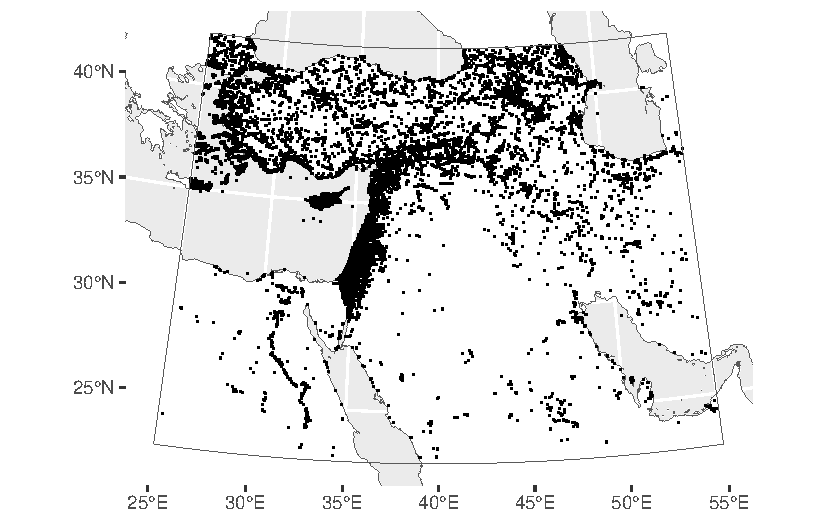
\includegraphics[keepaspectratio]{paper_files/figure-pdf/fig-occ-map-1.pdf}}

}

\caption{\label{fig-occ-map}Georeferenced occurrence records from West
Asia used to train models (N=1409939}

\end{figure}%

GBIF is currently the best available general-purpose occurrence dataset
for the West Asia region, its coverage is uneven both geographically and
from species to species. Figure~\ref{fig-occ-map} shows clearly that the
Southern Levant, and Israel specifically, is significantly more densely
sampled than other parts of West Asia.

Random Forest is a presence--absence approach to niche modelling and
therefore requires not just data on where a species is present, but
where it is definitely not present. However `absence' data is rarely
available because it requires exhaustive survey. In practice, most
applications of niche modelling are `presence-only' and, where absence
data is required (as for Random Forest), it is supplied as a random
background sample of points.\footnote{We use a background sample that is
  representative of the entire study area, as opposed to attempting to
  construct a `pseudo-absence' sample. See \citet{SilleroEtAl2021} for
  the distinction.} The purpose of this sample is to inform the model
about the nature of the underlying environment. The stochastic
generation process means that some of these points will overlap or fall
close to presences, so ensuring the model is not overly influenced by
background samples is critical to its predictive importance
\citep{ValaviEtAl2022}. Here we follow the advice of
\citet{BarbetMassinEtAl2012} for regression-based species distribution
models and use a large (≈10000) uniform sample of points from across the
land area of the study region. These points are then weighted equally
against the presences in the regression to produce a `balanced Random
Forest' \citep{ValaviEtAl2022}.

\subsection{Predictor data}\label{sec-predictors}

We modelled the occurrence of species as a function of 24 geospatial
predictor variables. These included:

\begin{verbatim}
bio_1, 
\end{verbatim}

\begin{verbatim}
Warning in CPL_read_gdal(as.character(x), as.character(options),
as.character(driver), : GDAL Message 1: dimension #0 (period) is not a Time or
Vertical dimension.
\end{verbatim}

\begin{verbatim}
Warning in parse_netcdf_meta(meta_data, get_names(x)): NAs introduced by
coercion
\end{verbatim}

\begin{verbatim}
bio_10, 
\end{verbatim}

\begin{verbatim}
Warning in CPL_read_gdal(as.character(x), as.character(options),
as.character(driver), : GDAL Message 1: dimension #0 (period) is not a Time or
Vertical dimension.
Warning in CPL_read_gdal(as.character(x), as.character(options),
as.character(driver), : NAs introduced by coercion
\end{verbatim}

\begin{verbatim}
bio_11, 
\end{verbatim}

\begin{verbatim}
Warning in CPL_read_gdal(as.character(x), as.character(options),
as.character(driver), : GDAL Message 1: dimension #0 (period) is not a Time or
Vertical dimension.
Warning in CPL_read_gdal(as.character(x), as.character(options),
as.character(driver), : NAs introduced by coercion
\end{verbatim}

\begin{verbatim}
bio_12, 
\end{verbatim}

\begin{verbatim}
Warning in CPL_read_gdal(as.character(x), as.character(options),
as.character(driver), : GDAL Message 1: dimension #0 (period) is not a Time or
Vertical dimension.
Warning in CPL_read_gdal(as.character(x), as.character(options),
as.character(driver), : NAs introduced by coercion
\end{verbatim}

\begin{verbatim}
bio_13, 
\end{verbatim}

\begin{verbatim}
Warning in CPL_read_gdal(as.character(x), as.character(options),
as.character(driver), : GDAL Message 1: dimension #0 (period) is not a Time or
Vertical dimension.
Warning in CPL_read_gdal(as.character(x), as.character(options),
as.character(driver), : NAs introduced by coercion
\end{verbatim}

\begin{verbatim}
bio_14, 
\end{verbatim}

\begin{verbatim}
Warning in CPL_read_gdal(as.character(x), as.character(options),
as.character(driver), : GDAL Message 1: dimension #0 (period) is not a Time or
Vertical dimension.
Warning in CPL_read_gdal(as.character(x), as.character(options),
as.character(driver), : NAs introduced by coercion
\end{verbatim}

\begin{verbatim}
bio_15, 
\end{verbatim}

\begin{verbatim}
Warning in CPL_read_gdal(as.character(x), as.character(options),
as.character(driver), : GDAL Message 1: dimension #0 (period) is not a Time or
Vertical dimension.
Warning in CPL_read_gdal(as.character(x), as.character(options),
as.character(driver), : NAs introduced by coercion
\end{verbatim}

\begin{verbatim}
bio_16, 
\end{verbatim}

\begin{verbatim}
Warning in CPL_read_gdal(as.character(x), as.character(options),
as.character(driver), : GDAL Message 1: dimension #0 (period) is not a Time or
Vertical dimension.
Warning in CPL_read_gdal(as.character(x), as.character(options),
as.character(driver), : NAs introduced by coercion
\end{verbatim}

\begin{verbatim}
bio_17, 
\end{verbatim}

\begin{verbatim}
Warning in CPL_read_gdal(as.character(x), as.character(options),
as.character(driver), : GDAL Message 1: dimension #0 (period) is not a Time or
Vertical dimension.
Warning in CPL_read_gdal(as.character(x), as.character(options),
as.character(driver), : NAs introduced by coercion
\end{verbatim}

\begin{verbatim}
bio_18, 
\end{verbatim}

\begin{verbatim}
Warning in CPL_read_gdal(as.character(x), as.character(options),
as.character(driver), : GDAL Message 1: dimension #0 (period) is not a Time or
Vertical dimension.
Warning in CPL_read_gdal(as.character(x), as.character(options),
as.character(driver), : NAs introduced by coercion
\end{verbatim}

\begin{verbatim}
bio_19, 
\end{verbatim}

\begin{verbatim}
Warning in CPL_read_gdal(as.character(x), as.character(options),
as.character(driver), : GDAL Message 1: dimension #0 (period) is not a Time or
Vertical dimension.
Warning in CPL_read_gdal(as.character(x), as.character(options),
as.character(driver), : NAs introduced by coercion
\end{verbatim}

\begin{verbatim}
bio_2, 
\end{verbatim}

\begin{verbatim}
Warning in CPL_read_gdal(as.character(x), as.character(options),
as.character(driver), : GDAL Message 1: dimension #0 (period) is not a Time or
Vertical dimension.
Warning in CPL_read_gdal(as.character(x), as.character(options),
as.character(driver), : NAs introduced by coercion
\end{verbatim}

\begin{verbatim}
bio_3, 
\end{verbatim}

\begin{verbatim}
Warning in CPL_read_gdal(as.character(x), as.character(options),
as.character(driver), : GDAL Message 1: dimension #0 (period) is not a Time or
Vertical dimension.
Warning in CPL_read_gdal(as.character(x), as.character(options),
as.character(driver), : NAs introduced by coercion
\end{verbatim}

\begin{verbatim}
bio_4, 
\end{verbatim}

\begin{verbatim}
Warning in CPL_read_gdal(as.character(x), as.character(options),
as.character(driver), : GDAL Message 1: dimension #0 (period) is not a Time or
Vertical dimension.
Warning in CPL_read_gdal(as.character(x), as.character(options),
as.character(driver), : NAs introduced by coercion
\end{verbatim}

\begin{verbatim}
bio_5, 
\end{verbatim}

\begin{verbatim}
Warning in CPL_read_gdal(as.character(x), as.character(options),
as.character(driver), : GDAL Message 1: dimension #0 (period) is not a Time or
Vertical dimension.
Warning in CPL_read_gdal(as.character(x), as.character(options),
as.character(driver), : NAs introduced by coercion
\end{verbatim}

\begin{verbatim}
bio_6, 
\end{verbatim}

\begin{verbatim}
Warning in CPL_read_gdal(as.character(x), as.character(options),
as.character(driver), : GDAL Message 1: dimension #0 (period) is not a Time or
Vertical dimension.
Warning in CPL_read_gdal(as.character(x), as.character(options),
as.character(driver), : NAs introduced by coercion
\end{verbatim}

\begin{verbatim}
bio_7, 
\end{verbatim}

\begin{verbatim}
Warning in CPL_read_gdal(as.character(x), as.character(options),
as.character(driver), : GDAL Message 1: dimension #0 (period) is not a Time or
Vertical dimension.
Warning in CPL_read_gdal(as.character(x), as.character(options),
as.character(driver), : NAs introduced by coercion
\end{verbatim}

\begin{verbatim}
bio_8, 
\end{verbatim}

\begin{verbatim}
Warning in CPL_read_gdal(as.character(x), as.character(options),
as.character(driver), : GDAL Message 1: dimension #0 (period) is not a Time or
Vertical dimension.
Warning in CPL_read_gdal(as.character(x), as.character(options),
as.character(driver), : NAs introduced by coercion
\end{verbatim}

\begin{verbatim}
bio_9, 
\end{verbatim}

\begin{verbatim}
Warning in CPL_read_gdal(as.character(x), as.character(options),
as.character(driver), : GDAL Message 1: dimension #0 (period) is not a Time or
Vertical dimension.
Warning in CPL_read_gdal(as.character(x), as.character(options),
as.character(driver), : NAs introduced by coercion
\end{verbatim}

\begin{itemize}
\tightlist
\item
  Sixteen `bioclimatic' variables derived from monthly temperature and
  precipitation values, following standard practice for species
  distribution models \citep{HijmansEtAl2005}. Contemporary bioclimatic
  predictor data for West Asia was extracted from the global CHELSA
  dataset \citep{KargerEtAl2017}, which predicts temperature and
  precipitation from downscaled general circulation model output at 1 km
  resolution.
\end{itemize}

\begin{itemize}
\tightlist
\item
  Terrain aspect and slope, which at high resolution perform well as
  proxies for solar radiation when modelling plant occurrence
  \citep{AustinVanNiel2011, LeempoelEtAl2015}; and the topographic
  wetness index (TWI), which serves as a proxy for soil moisture and is
  particularly important in modelling arid environments
  \citep{KopeckyCizkova2010, CamposEtAl2016, DiVirgilioEtAl2018}. All
  three were derived from the SRTM30+ digital elevation model using
  algorithms from WhiteboxTools \citep{Lindsay2016}.
\end{itemize}

\begin{itemize}
\tightlist
\item
  Edaphic data from SoilGrids \citep{HenglEtAl2014, HenglEtAl2017},
  which improves model performance for plants
  \citep{DubuisEtAl2013, ModEtAl2016, VelazcoEtAl2017}. Based on a
  recent assessment of the reliability of SoilGrids data for species
  distribution modelling \citep{MillerEtAl2024}, we used a subset of
  four variables relating to soil texture (clay, silt, sand) and pH at
  the surface (0-5 cm depth).
\end{itemize}

For hindcasting, we used reconstructed bioclimatic data for three key
climatologies generated from downscaled paleoclimate simulations from
the HadCM3 general circulation model
\citep{FordhamEtAl2017, BrownEtAl2018}: the Bølling--Allerød
(c.~14.7--12.9 ka), the Younger Dryas (c.~12.9--11.7 ka), and the Early
Holocene (11.7--8.3 ka). Terrain and soil predictors were held constant,
since reconstructions of these variables in the past are not available
at sufficient scale. It is unlikely that either macroscale topography or
soil characteristics have altered significantly over the period of time
considered here, so we assume that this does not degrade model
performance, and may in fact benefit it by providing `anchoring'
predictors that are independent of climate change.

For training, test predictions, and archaeological predictions predictor
data was left in its native projection and resolution. For hindcast
palaeodistributions, it was transformed to common equal-area projection
and resolution of 5 km.

\begin{verbatim}
Warning: There were 57 warnings in `mutate()`.
The first warning was:
i In argument: `occ = map(occ, bind_extract, st_as_stars(hack(climate,
  "period", "cur")))`.
Caused by warning in `CPL_get_metadata()`:
! GDAL Message 1: dimension #0 (period) is not a Time or Vertical dimension.
i Run `dplyr::last_dplyr_warnings()` to see the 56 remaining warnings.
\end{verbatim}

\subsection{Random Forest}\label{random-forest}

Ecological niche modelling is a classification problem that can be
approached with a wide range of statistical methods. A substantial
literature exists on the relatively performance of these approaches and
their respective parameterisations \citep[reviewed
in][]{ValaviEtAl2022}. Random Forest, a widely-used machine learning
algorithm, is amongst the best performing methods for presence-only
species distribution models, providing it is appropriately parameterised
to account for the class imbalance between presence and background
samples \citep{ValaviEtAl2021, ValaviEtAl2022}. For our application, it
also has the advantage of requiring little to no manual parameter tuning
to achieve good predictive results, which makes it easier to model a
larger numbers of taxa.

For each taxon we trained a classification model to predict occurrence
(presence or absence/background) based on up to 24 predictor variables
(Section~\ref{sec-predictors}). Highly correlated (Pearson's
\emph{r}\textgreater0.7) predictors were removed on a taxon-by-taxon
basis, to mitigate issues of overfitting due to colinearity
\citep{DormannEtAl2013}, as were redundant predictors with zero
variance. We used the Random Forest algorithm implemented in the R
package `ranger' \citep{WrightZiegler2017} and the `tidymodels'
\citep{tidymodels} framework for data preprocessing and model selection.
To avoid overfitting, we follow \citet{ValaviEtAl2021} in their
recommended hyperparameters and use of down-sampling to balance presence
and background samples. Models for each taxon were fit independently,
with redundant zero-variance predictors excluded, and assessed based on
balanced training (¾) and test (¼) partitions.

\section{Model assessment}\label{model-assessment}

We trained Random Forest models for 63 taxa using contemporary
occurrence data from GBIF, a random sample of background points, and the
predictor variables described in Section~\ref{sec-predictors}.
Substituting the ``current'' climate predictors for those derived from
palaeoclimatic simulations \citep{BrownEtAl2018}, we could then generate
hindcast predictions for reconstructed past environments in 4 key
climate periods -- a total of 252 modelled palaeodistributions.
Predicted distributions for individual taxa are presented in the
appendix and accompanying material.

\begin{figure}

\centering{

\pandocbounded{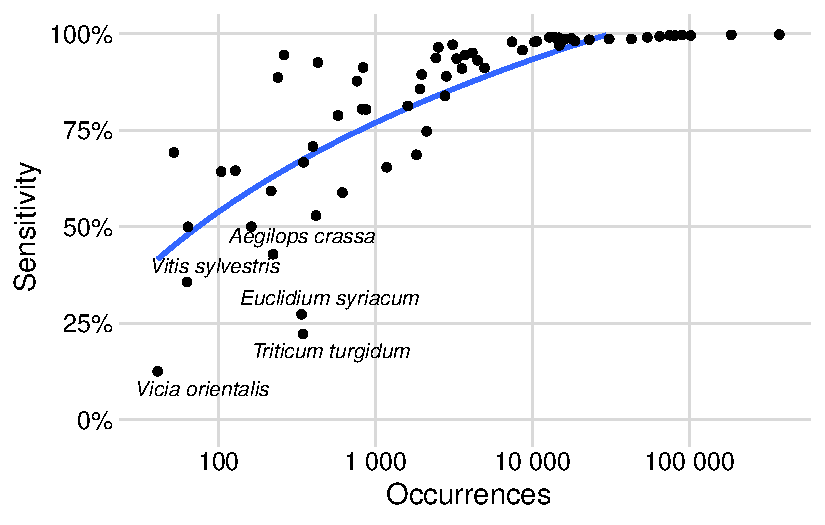
\includegraphics[keepaspectratio]{paper_files/figure-pdf/fig-model-sensitivity-vs-n_occ-1.pdf}}

}

\caption{\label{fig-model-sensitivity-vs-n_occ}Model sensitivity by
number of training occurrences}

\end{figure}%

We assessed the predictive performance of the fitted niche models in the
contemporary environment based on the reserved test partition
Table~\ref{tbl-results-summary}. Model accuracy (proportion of correctly
classified presence and background samples) ranged between 92\% and
100\%, with an average of 97\%. Sensitivity (proportion of correctly
classified presence samples) ranged between 12\% and 100\%, with an
average of 82\%. The area under the models' receiver operating
characteristic curves (ROC-AUC) was on average 0.987±0.018 Model
sensitivity is loosely correlated with the number of occurrences
available for training (Figure~\ref{fig-model-sensitivity-vs-n_occ}),
with the worst-performing models all having less than 300 recorded
occurrences: \emph{Lathyrus sativus}, \emph{Lepidium perfoliatum},
\emph{Triticum aestivum}, \emph{Bolboschoenus glaucus}, \emph{Gypsophila
vaccaria}, \emph{Euclidium syriacum}, \emph{Gypsophila elegans},
\emph{Citrullus colocynthis}, \emph{Triticum monococcum}, \emph{Triticum
turgidum}, \emph{Aegilops crassa}, \emph{Secale strictum}, \emph{Cicer
reticulatum}, \emph{Medicago astroites}, \emph{Triticum durum},
\emph{Gypsophila pilosa}, \emph{Arnebia decumbens}, \emph{Salvia
absconditiflora}, \emph{Suaeda fruticosa}, \emph{Buglossoides
tenuiflora}, \emph{Lathyrus oleraceus}, \emph{Vitis sylvestris}, and
\emph{Vicia orientalis}. Test metrics and ROC curves for the individual
models are included in the appendix.

The ability of the hindcast models to predict the occurrence of specific
species at archaeological sites is worse, with 10\% of presences in
archaeobotanical assemblages successfully predicted. Model sensitivity
(proportion of corrected predicted presenses) in relation to the
archaeological data is on average 0.07±0.15
Table~\ref{tbl-results-summary}. A full assessment of the hindcasting
performance of the individual models can be found in the appendix.

\begingroup
\setlength\LTleft{0\linewidth}
\setlength\LTright{0\linewidth}\fontsize{8.2pt}{9.9pt}\selectfont
\setlength{\LTpost}{0mm}

\begin{longtable}{@{\extracolsep{\fill}}lrrrrrr}

\caption{\label{tbl-results-summary}Summary of species modelled}

\tabularnewline

\toprule
 & \multicolumn{2}{c}{Occurrences} & \multicolumn{4}{c}{Model} \\ 
\cmidrule(lr){2-3} \cmidrule(lr){4-7}
Taxon & Arch. & Cur. & Acc. & ROC-AUC & Sens. & Sens. (arch.) \\ 
\midrule\addlinespace[2.5pt]
{\itshape Aegilops crassa} & 4 & 223 & 0.98 & 0.98 & 0.43 & 0.00 \\ 
{\itshape Aizoanthemopsis hispanica}\textsuperscript{\textit{1}} & 4 & 762 & 0.99 & 1.00 & 0.88 & 0.50 \\ 
{\itshape Ammi majus} & 4 & 10311 & 0.97 & 0.99 & 0.98 & 0.00 \\ 
{\itshape Androsace maxima} & 17 & 4946 & 0.94 & 0.98 & 0.91 & 0.06 \\ 
{\itshape Arenaria serpyllifolia} & 3 & 101612 & 0.98 & 0.98 & 1.00 & 0.00 \\ 
{\itshape Arnebia decumbens} & 21 & 616 & 0.97 & 0.97 & 0.59 & 0.05 \\ 
{\itshape Arnebia linearifolia} & 13 & 239 & 1.00 & 0.99 & 0.89 & 0.00 \\ 
{\itshape Atriplex prostrata} & 4 & 80181 & 0.98 & 0.99 & 1.00 & 0.00 \\ 
{\itshape Avena sterilis} & 5 & 15906 & 0.96 & 0.99 & 0.99 & 0.40 \\ 
{\itshape Bassia arabica} & 4 & 262 & 1.00 & 1.00 & 0.95 & 0.00 \\ 
{\itshape Bolboschoenus glaucus} & 5 & 418 & 0.98 & 0.97 & 0.53 & 0.00 \\ 
{\itshape Bolboschoenus maritimus}\textsuperscript{\textit{2}} & 31 & 53809 & 0.98 & 1.00 & 0.99 & 0.00 \\ 
{\itshape Brachypodium distachyon} & 5 & 13800 & 0.98 & 1.00 & 0.99 & 0.20 \\ 
{\itshape Bromus sterilis} & 3 & 89764 & 0.99 & 0.99 & 1.00 & 0.00 \\ 
{\itshape Buglossoides arvensis} & 23 & 23004 & 0.95 & 0.98 & 0.98 & 0.09 \\ 
{\itshape Buglossoides tenuiflora} & 26 & 399 & 0.99 & 0.99 & 0.71 & 0.04 \\ 
{\itshape Capparis spinosa} & 4 & 8617 & 0.97 & 0.99 & 0.96 & 0.00 \\ 
{\itshape Carex divisa} & 9 & 7400 & 0.97 & 0.99 & 0.98 & 0.00 \\ 
{\itshape Chenopodium album} & 5 & 184403 & 0.99 & 0.98 & 1.00 & 0.00 \\ 
{\itshape Cicer reticulatum}\textsuperscript{\textit{3}} & 3 & 52 & 1.00 & 1.00 & 0.69 & 0.00 \\ 
{\itshape Citrullus colocynthis} & 4 & 1823 & 0.94 & 0.95 & 0.69 & 0.00 \\ 
{\itshape Crithopsis delileana} & 3 & 430 & 1.00 & 1.00 & 0.93 & 0.00 \\ 
{\itshape Euclidium syriacum} & 3 & 338 & 0.98 & 0.97 & 0.27 & 0.00 \\ 
{\itshape Ficus carica} & 8 & 64424 & 0.98 & 0.99 & 0.99 & 0.38 \\ 
{\itshape Fumaria densiflora} & 4 & 3704 & 0.96 & 0.99 & 0.94 & 0.00 \\ 
{\itshape Gypsophila elegans} & 3 & 1603 & 0.95 & 0.98 & 0.81 & 0.00 \\ 
{\itshape Gypsophila pilosa} & 5 & 348 & 0.99 & 0.99 & 0.67 & 0.00 \\ 
{\itshape Gypsophila vaccaria}\textsuperscript{\textit{4}} & 8 & 1177 & 0.95 & 0.98 & 0.65 & 0.00 \\ 
{\itshape Henrardia pubescens} & 3 & 1\textsuperscript{\textit{5}} & — & — & — & — \\ 
{\itshape Hordeum bulbosum} & 4 & 4134 & 0.97 & 1.00 & 0.95 & 0.00 \\ 
{\itshape Hordeum murinum} & 5 & 74770 & 0.98 & 0.99 & 1.00 & 0.00 \\ 
{\itshape Hordeum spontaneum}\textsuperscript{\textit{6}} & 76 & 3098 & 0.99 & 1.00 & 0.97 & 0.20 \\ 
{\itshape Lathyrus aphaca} & 4 & 18652 & 0.96 & 0.99 & 0.98 & 0.00 \\ 
{\itshape Lathyrus oleraceus}\textsuperscript{\textit{7}} & 8 & 819 & 0.98 & 0.99 & 0.80 & 0.00 \\ 
{\itshape Lathyrus sativus} & 4 & 2120 & 0.92 & 0.96 & 0.75 & 0.00 \\ 
{\itshape Lepidium perfoliatum} & 3 & 2764 & 0.94 & 0.98 & 0.84 & 0.00 \\ 
{\itshape Linum bienne}\textsuperscript{\textit{8}} & 14 & 12824 & 0.98 & 0.99 & 0.99 & 0.07 \\ 
{\itshape Lolium rigidum} & 5 & 10620 & 0.97 & 0.99 & 0.98 & 0.00 \\ 
{\itshape Lolium temulentum} & 3 & 4463 & 0.94 & 0.98 & 0.93 & 0.00 \\ 
{\itshape Medicago astroites}\textsuperscript{\textit{9}} & 15 & 104 & 1.00 & 0.99 & 0.64 & 0.00 \\ 
{\itshape Medicago radiata} & 20 & 834 & 0.99 & 0.99 & 0.91 & 0.30 \\ 
{\itshape Phalaris paradoxa} & 3 & 3287 & 0.97 & 0.99 & 0.94 & 0.00 \\ 
{\itshape Phragmites australis} & 4 & 373041 & 0.99 & 0.99 & 1.00 & 0.00 \\ 
{\itshape Pistacia atlantica} & 6 & 2419 & 0.99 & 1.00 & 0.94 & 0.33 \\ 
{\itshape Poa bulbosa} & 5 & 30769 & 0.96 & 0.98 & 0.99 & 0.20 \\ 
{\itshape Polygonum arenarium}\textsuperscript{\textit{10}} & 7 & 25\textsuperscript{\textit{5}} & — & — & — & — \\ 
{\itshape Polygonum corrigioloides} & 6 & 12\textsuperscript{\textit{5}} & — & — & — & — \\ 
{\itshape Prosopis farcta} & 5 & 2512 & 0.99 & 1.00 & 0.96 & 0.60 \\ 
{\itshape Rumex pulcher} & 6 & 17606 & 0.97 & 0.99 & 0.99 & 0.00 \\ 
{\itshape Salsola kali} & 6 & 14699 & 0.98 & 1.00 & 0.99 & 0.00 \\ 
{\itshape Salvia absconditiflora}\textsuperscript{\textit{11}} & 3 & 128 & 0.99 & 1.00 & 0.65 & 0.00 \\ 
{\itshape Secale cereale} & 4 & 14803 & 0.95 & 0.98 & 0.97 & 0.00 \\ 
{\itshape Secale strictum}\textsuperscript{\textit{12}} & 3 & 162 & 0.99 & 0.99 & 0.50 & 0.00 \\ 
{\itshape Suaeda fruticosa} & 3 & 577 & 0.99 & 1.00 & 0.79 & 0.00 \\ 
{\itshape Taeniatherum caput-medusae} & 4 & 1969 & 0.96 & 0.99 & 0.89 & 0.00 \\ 
{\itshape Triticum aestivum}\textsuperscript{\textit{13}} & 4 & 217 & 0.99 & 0.98 & 0.59 & 0.00 \\ 
{\itshape Triticum durum} & 3 & 64 & 1.00 & 0.99 & 0.50 & 0.00 \\ 
{\itshape Triticum monococcum}\textsuperscript{\textit{14}} & 47 & 870 & 0.98 & 0.99 & 0.80 & 0.15 \\ 
{\itshape Triticum turgidum}\textsuperscript{\textit{15}} & 53 & 345 & 0.97 & 0.93 & 0.22 & 0.00 \\ 
{\itshape Verbena officinalis} & 3 & 89654 & 0.99 & 0.99 & 1.00 & 0.00 \\ 
{\itshape Vicia ervilia} & 26 & 1924 & 0.95 & 0.98 & 0.86 & 0.35 \\ 
{\itshape Vicia faba} & 7 & 42636 & 0.97 & 0.99 & 0.99 & 0.43 \\ 
{\itshape Vicia narbonensis}\textsuperscript{\textit{16}} & 3 & 2826 & 0.95 & 0.99 & 0.89 & 0.33 \\ 
{\itshape Vicia orientalis}\textsuperscript{\textit{17}} & 16 & 41 & 1.00 & 0.95 & 0.12 & 0.00 \\ 
{\itshape Vitis sylvestris} & 3 & 63 & 1.00 & 0.99 & 0.36 & 0.00 \\ 
{\itshape Zygophyllum fabago} & 3 & 3554 & 0.97 & 0.99 & 0.91 & 0.00 \\ 
\bottomrule

\end{longtable}

\begin{minipage}{\linewidth}
\textsuperscript{\textit{1}}Including \emph{Aizoon hispanicum}\\
\textsuperscript{\textit{2}}Including \emph{Scirpus maritimus}\\
\textsuperscript{\textit{3}}Including \emph{Cicer arietinum}\\
\textsuperscript{\textit{4}}Including \emph{Vaccaria pyramidata}\\
\textsuperscript{\textit{5}}Excluded from modelling due to sample size\\
\textsuperscript{\textit{6}}Including \emph{Hordeum vulgare}\\
\textsuperscript{\textit{7}}Including \emph{Pisum sativum} and \emph{Pisum elatius}\\
\textsuperscript{\textit{8}}Including \emph{Linum usitatissimum}\\
\textsuperscript{\textit{9}}Including \emph{Trigonella astroites}\\
\textsuperscript{\textit{10}}Including \emph{Polygonum venantianum}\\
\textsuperscript{\textit{11}}Including \emph{Salvia cryptantha}\\
\textsuperscript{\textit{12}}Including \emph{Secale montanum}\\
\textsuperscript{\textit{13}}Including \emph{Triticum spelta} and \emph{Triticum aestivocompactum}\\
\textsuperscript{\textit{14}}Including \emph{Triticum boeoticum}\\
\textsuperscript{\textit{15}}Including \emph{Triticum aestivum}, \emph{Triticum dicoccum}, and \emph{Triticum dicoccoides}\\
\textsuperscript{\textit{16}}Including \emph{Vicia narbonense}\\
\textsuperscript{\textit{17}}Including \emph{Lens culinaris} and \emph{Lens orientalis}\\
\end{minipage}
\endgroup

\section{Discussion}\label{discussion}

\subsection{Reduction in range sizes over the Pleistocene/Holocene
boundary}\label{reduction-in-range-sizes-over-the-pleistoceneholocene-boundary}

\begin{figure}

\centering{

\pandocbounded{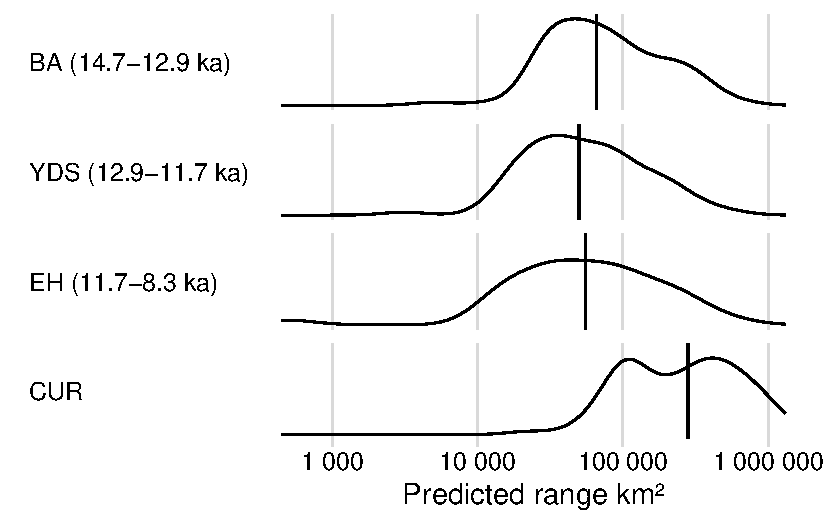
\includegraphics[keepaspectratio]{paper_files/figure-pdf/fig-pred-range-density-1.pdf}}

}

\caption{\label{fig-pred-range-density}Distribution of predicted species
ranges by period. Dashed lines indicate the median range.}

\end{figure}%

Our reconstructed palaeodistributions (shown in full in the appendix)
indicate that the majority of species had significantly different
geographic ranges in the Late Pleistocene/Early Holocene compared today.
55 of 63 species are predicted reduced ranges in the past; 54 of more
than 10\% or more. Though the magnitude of the change in range size from
prehistory to the present likely reflects a degree of overfitting in the
model (discussed further in Section~\ref{sec-discuss-hindcasting}),
fluctuations in modelled range size between the Bølling-Allerød
(14.7--12.9 ka), Younger Dryas (12.9--11.7 ka), and Early Holocene
(11.7--8.3 ka) are more directly comparable
(Figure~\ref{fig-pred-range-density}). The average range of modelled
species was 31\% in the Early Holocene compared to the Bølling--Allerød,
and 28\% during the Younger Dryas (i.e.~ranges recovered slightly
between the Younger Dryas and Early Holocene). This perhaps indicates
that although this period is considered one of climatatic amelioration
globally \citep{JonesEtAl2019}, the colder conditions of the Pleistocene
may have supported more extensive plant-based economies in West Asia
specifically.

\begin{figure}

\centering{

\pandocbounded{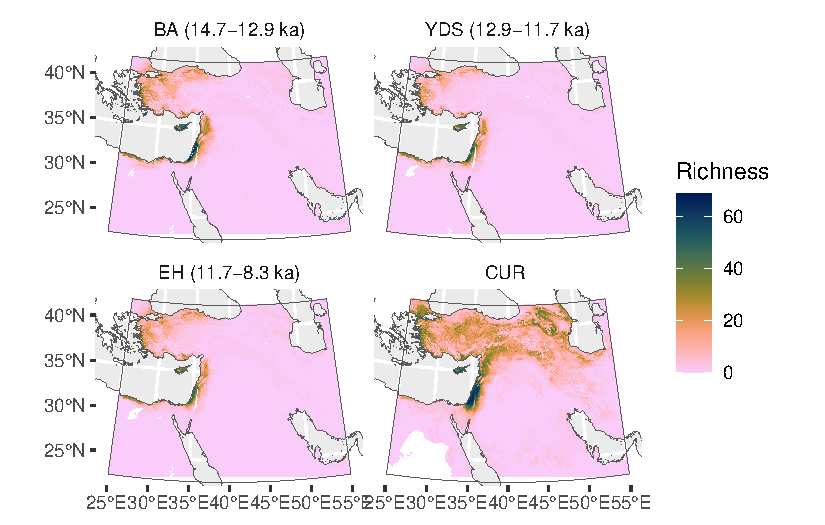
\includegraphics[keepaspectratio]{paper_files/figure-pdf/fig-palaeodist-sum-1.pdf}}

}

\caption{\label{fig-palaeodist-sum}Predicted species richness (sum of
predicted ranges) by period}

\end{figure}%

Many taxa that occur (or are predicted to occur) across the `hilly
flanks' today---including most crop progenitors---are reconstructed to
have had a significantly more restricted distribution in the terminal
Pleistocene/Early Holocene (Figure~\ref{fig-palaeodist-sum}). These
include \emph{Ficus carica} (fig); \emph{Hordeum} spp. (wild barleys);
\emph{Lathyrus aphaca} and \emph{L. sativus} (both marginally edible
legumes); \emph{Triticum aestivum compactum} (in the N. Levant),
\emph{T. monococcum aegilopoides}, \emph{T. durum}, and \emph{Triticum
urartu} (but not the other wheat progenitor, \emph{T. turgidum dicoccum}
-- see Section~\ref{sec-discuss-crops}); \emph{Aegilops speltoides}, but
not \emph{Aegilops tauschii} (goatgrasses); and \emph{Vicia} spp.
(vetches), including \emph{Vicia faba} (broad beans). Most of Anatolia,
Northern Mesopotamia, and the Zagros Mountains in particular disappear
from the predicted ranges of these species, leaving the Levant and to a
lesser extent the Aegean and Cyprus as refugia.

Our results for the Levant are consistent with the current understanding
of this region as developing early intensive foraging economies
\citep[the Natufian culture,][]{BarYosef1998} and as a centre of origin
of agriculture \citep{Zeder2011a}. Within the Levant, many species show
moderate reductions in ranges over the Pleistocene/Holocence boundary,
retreating from the Badia/transjordan region (e.g.~barley, fig.
\textbf{?@fig-palaeodist-barely-levant}).

Loss of the Northern Mesopotamia--Anatolia region from the predicted
ranges of crop progenitors is interesting in light of the `golden
triangle' hypothesis
\citep{Lev-YadunEtAl2000, KozlowskiAurenche2005, AbboEtAl2010}, which
puts this region at the centre of the development of agriculture and
plant domestication. Multiple lines of archaeological evidence have
emerged that point away from this hypothesis and towards a more
geographically diverse origin
\citep{Asouti2006, FullerEtAl2011, ArranzOtaeguiEtAl2016}, and our
reconstructions are also consistent with the late arrival of intensive
plant-based foraging economies in this region (cf.~the Natufian of the
Levant).

The near-absence of the Zagros in any predicted ranges is also
surprising, given mounting evidence that animal domestication took place
just as early in the eastern \emph{Mashriq} as it did in the west
\citep{Zeder2024}. We consider that the most likely explanation for this
is that our flora does not include the species that were most important
to plant subsistence in the east. Archaeobotanical data on Neolithic
sites in the Zagros is limited (compared to the Levant in particular)
due to a hiatus in field research there from the 1980s to early 2010s
\citep{Zeder2024}. Recent research
\citep{RiehlEtAl2013, WeideEtAl2017, WeideEtAl2018, WhitlamEtAl2018, GonzalezCarreteroEtAl2023}
indicates that plant subsistence in this region was based on a distinct
set of species, compared to the Levant and Anatolia.

Cyprus and the Aegean are not conventionally considered part of the
primary zone of domestication but rather amongst the first regions that
acquired agriculture from West Asia. Our analysis complicates this
picture, as it indicates that the wild ranges of many crop progenitors
included these regions. Early examples of several domesticates are
recorded at sites on Cyprus, Western Anatolia and Greece
\citep{ArranzOtaeguiRoe2023}, and the Aegean region was probably
connected to West Asia by a land bridge via Anatolia until the Early
Holocene \citep{AksuHiscott2022}. Were these area part of the same
broader `interaction sphere' that produce Neolithic agriculture in West
Asia?

Exceptions to the dominant trend of range reduction include \emph{Cicer
reticulatum} (wild chickpea), which has a relatively stable range
centered on Northern Mesopotamia; and \emph{Triticum turgidum dicoccum}
(wild emmer wheat), which is predicted to have two limited ranges
centered around the Black Sea Coast of Anatolia and the Palmyra basin.
In the latter case, neither of these areas are part of the predicted (by
our model) modern distribution of wild emmer, which is centered around
the Caucasus and Northern Mesopotamia. But it would be consistent with
archaeological evidence for early cultivation at sites in the Upper
Euphrates \citep{Willcox2024}.

\subsection{Biogeography of crop progenitors}\label{sec-discuss-crops}

\begin{figure}

\centering{

\pandocbounded{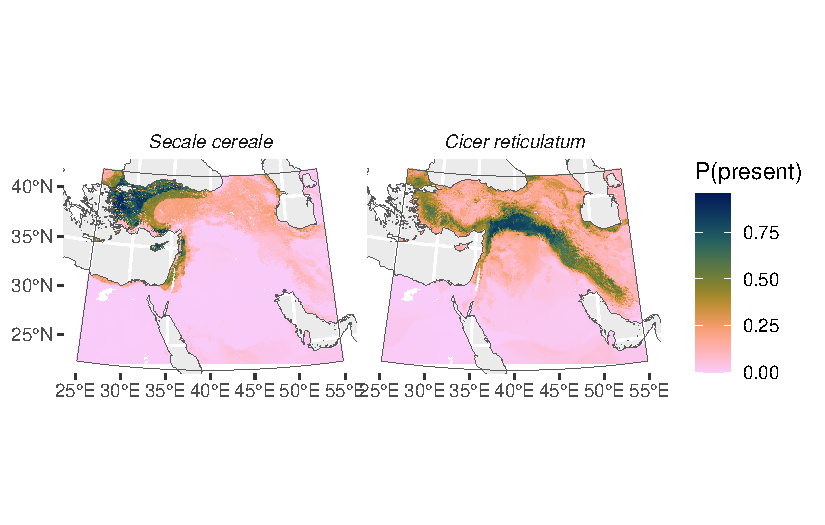
\includegraphics[keepaspectratio]{paper_files/figure-pdf/fig-palaeodist-chickpea-rye-1.pdf}}

}

\caption{\label{fig-palaeodist-chickpea-rye}Predicted palaeodistribution
of wild chickpea and rye in the Early Holocene (11.7--8.2 ka)}

\end{figure}%

Almost all the cereal and legume crop progenitors we modelled are
predicted to have only been found in the Levant during the terminal
Pleistocene and Early Holocene (see appendix). Part of this may be do
with the fact that both our initial flora and training occurrence
dataset have a strong bias towards the southern Levant, but strikingly
the modelled \emph{current} ranges of these plants do tend to include
Anatolia and the Zagros, so this cannot be the only factor. One notable
exception is the wild ancestor of chickpea (\emph{Cicer reticulatum}),
which is predicted to have a distribution centered on Northern
Mesopotamia but encompassing much of the the `hilly flanks' (except the
southern Levant, Figure~\ref{fig-palaeodist-chickpea-rye}). Another is
rye (\emph{Secale cereale}), which is inferred to be primarily Anatolian
(Figure~\ref{fig-palaeodist-chickpea-rye}). This is perhaps relevant to
rye's unusual domestication history, as a crop of West Asian origin that
was intensively exploited \citep{HillmanEtAl2001, DoucheWillcox2018} but
apparently not first cultivated until much later than the `founder
crops', in Europe \citep{SchreiberEtAl2021}.

\begin{figure}

\centering{

\pandocbounded{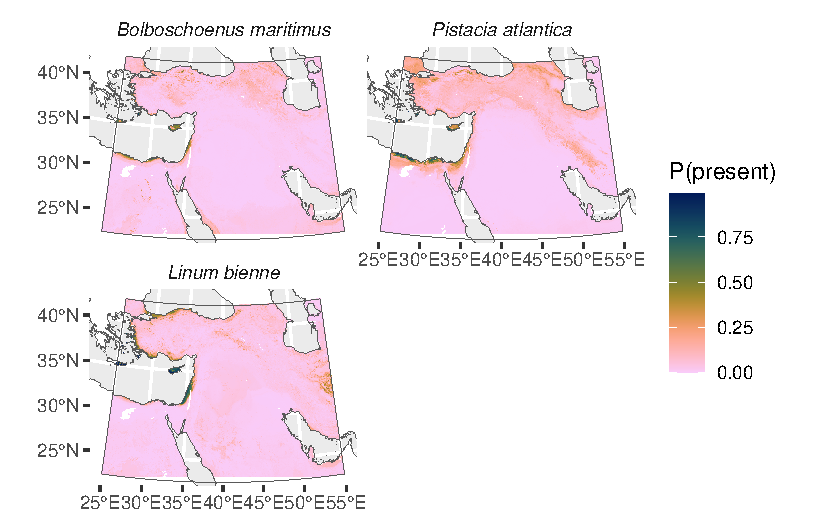
\includegraphics[keepaspectratio]{paper_files/figure-pdf/fig-palaeodist-locals-1.pdf}}

}

\caption{\label{fig-palaeodist-locals}Predicted palaeodistribution of
flax, pistachio and clubrush in the Early Holocene (11.7--8.2 ka)}

\end{figure}%

Flax (\emph{Linum bienne}) is predicted to have had a highly
concentrated distribution in Cyprus and along the Mediterranean coast of
the southern Levant. This is consistent with its low ubiquity in
archaeobotanical assemblages \citep{ArranzOtaeguiRoe2023}, despite
conventionally being considered a `founder crop', and presumably implies
that its domestication was similarly geographically constrained. It is
the only unambiguous crop progenitor with such a restricted range,
though pistachio (\emph{Pistacia atlantica}) and clubrush
(\emph{Bolboschoenus maritimus}) are similarly constrained to the
Mediterranean coast (and North Africa, in the case of pistachio). This
is despite the fact that they are well-attested in the archaeotanical
record from across West Asia.

Wild barley (\emph{Hordeum spontaneum}) its relatives show a contraction
of their predicted ranges from the Pleistocene to the Holocene,
concurrent with it being brought into cultivation
(\textbf{?@fig-palaeodist-barely-levant}). It also sees a marked decline
in the archaeobotanical record from the Early PPNA/Early PPNB (where it
was amongst the most common taxa) to the Late PPNB and Late Neolithic
\citep{ArranzOtaeguiRoe2023}. Pistachio (\emph{Pistacia atlantica})
shows similar trends, but it is less certain that this species was
managed in the Neolithic. Conversely, the various wild wheat species
native to West Asia show almost no response to Pleistocene/Holocene
climate change, even within the Levant, and in the archaeobotanical
record wheat displays the opposite trend to barley and pistachio --
becoming gradually more abundant through the course of the Neolithic and
dominant by its end \citep{ArranzOtaeguiRoe2023}.

\begin{figure}

\centering{

\pandocbounded{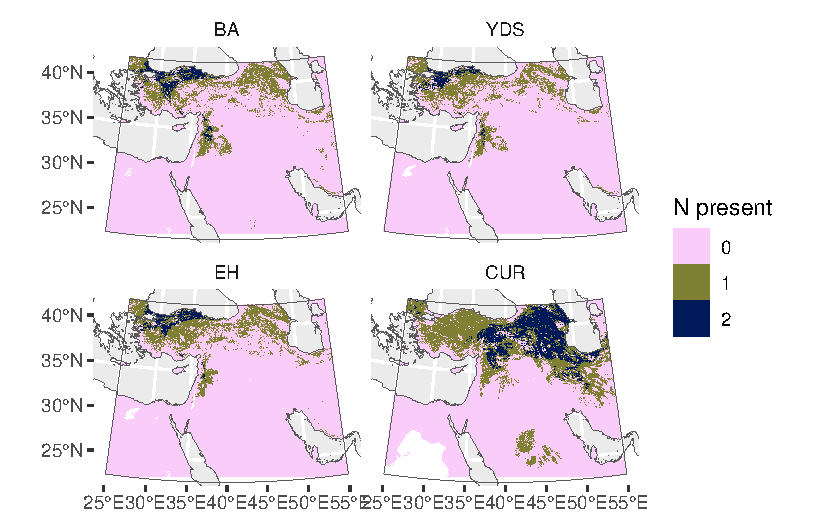
\includegraphics[keepaspectratio]{paper_files/figure-pdf/fig-palaeodist-bread-1.pdf}}

}

\caption{\label{fig-palaeodist-bread}Combined predicted
palaeodistributions of bread wheat progenitors}

\end{figure}%

Bread wheat (\emph{Triticum aestivum}), the most common wheat cultivar
today, has a complex ancestry that involves two recent hybridisation
events \citep{LevyFeldman2022}: most recently between domestic emmer
(\emph{Triticum turgidum dicoccum}) and a goatgrass (\emph{Aegilops
tauschii}) c.~9 ka, and before that, in emmer, between wild red einkorn
(\emph{T. urartu}) and another goatgrass (\emph{Aegilops speltoides}).
Although there is fairly wide overlap between these species today,
according to our modelling the only place all four (or even just three)
are predicted to have coincided or been found in close proximity to each
other in the time frame of domestication is a narrow area around the
Orontes river in the northern Levant
(Figure~\ref{fig-palaeodist-bread}). This area is c.~200 km from the
only two sites in our archaeobotanical database where bread wheat
(\emph{T. aestivum}) co-occurs with both of its recent progenitors
(\emph{A. tauschii} and \emph{T. turgidum dicoccum}) or both species of
wheat and the goatgrasses are found together: Tell Abu Hureyra and El
Kowm II \citep{ArranzOtaeguiRoe2023}.\footnote{We are grateful to
  Benjamin Nowak for pointing this out to us.} Taken together this
suggests an origin of domesticated bread wheat, otherwise only loosely
geographically constrained to the Levant--Upper Euphrates corridor
\citep{LevyFeldman2022}, is possibly occurred in this vicinity.

\subsection{Hindcast models do not predict archaeobotanical
composition}\label{sec-discuss-hindcasting}

The failure of our hindcast models to predict the occurrence of species
in archaeobotanical assemblages has several possible explanations. Since
they do accurately predict the test dataset, a likely culprit is
overfitting of the models to the present environment. This implies that
the modelled palaeodistributions should be seen as conservative
estimates or a minimal range. Another obvious flaw in our methodology is
that the time slices used for palaeoclimatic reconstruction are very
broad---each covering around two millennia---and therefore potentially
unrepresentative of the environment around sites at the specific time at
which they were occupied. The variable quality of the archaeological
test dataset, especially in terms of chronology, is also a plausible
factor.

For a variety of reasons, our models almost certainly underestimate the
\emph{fundamental} niche or potential distribution of the target taxon.
These include:

\begin{itemize}
\tightlist
\item
  The uneven coverage of the GBIF occurrence dataset (see
  Section~\ref{sec-occ-data})
\end{itemize}

At the same time, we cannot rule out more substantive reasons for the
discrepency between predicted and observed archaeological occurrences.
The niches of the modelled species could have changed since the Early
Holocene, which would not be captured in a model trained purely on
modern specimens. Human economic choices---mobility, foraging
strategies, cultivation, etc.---could also produce archaeobotanical
assemblages whose composition depart significantly from that of the
surrounding local flora. Further refinement of the methodology for
hindcast palaeoecological niche models, for example using more finely
resolved palaeoclimate sequences \citep[e.g.][]{KargerEtAl2023},
hyperparameter tuning to avoid overfitting, and improved archaeological
datasets, would help disentangle these potential explanations.

\section{Conclusion}\label{conclusion}

We present the first continuous, spatially explicit models of the
palaeodistributions of 63 plant species found regularly in association
with Late Epipalaeolithic and Early Neolithic sites in West Asia. This
deductive approach---modelling the niche of a species based on its
occurrence in relation to environmental factors today, and using this
together with palaeoclimate simulations to infer its past
distribution---represents a new line of evidence on the archaeoecology
of the world's first agricultural societies. It provides a complementary
picture to that gleaned from environmental archaeology and
climatological archives because it is independent of the taphonomic,
anthropic, and recovery-related processes that affect these records.

``All models are wrong'' \citep{Box1976}, but the performance of our
models on independent test datasets give confidence in its predictions,
which are plausible and consistent with broad-scale patterns in the
archaeological record. Results with regard to specific
archaeologically-attested species are not as promising, but this also
reflects the incomplete and coarsely temporally-resolved nature of the
archaeobotanical verification dataset. Discrepancies between the
modelled distribution, whether on the broad scale (e.g.~the restricted
geographic range of most species compared to their attestation in the
archaeological record), or relating to specific species (i.e.~false
positives and false negatives), suggest several avenues for future
investigation.

Modelling a large number of species using machine learning, the
substantial occurrence datasets available for the present day, and a
hindcasting approach to past distributions also represents a significant
advance in the methodology of palaeoecological niche modelling. This
approach is enabled by the availability of high quality, global open
datasets in ecology \citep{GBIF2025, GBIFSecretariat2023}, earth science
\citep{SRTM}, and climatology \citep{KargerEtAl2017, BrownEtAl2018}.
Unfortunately in relation to these fields open data in archaeology lags
conspiciously behind. Though we have benefited from the relatively long
tradition of compiling archaeobotanical data in our region of study
\citep{ColledgeEtAl2004, ShennanConolly2007, ADEMNES, LucasFuller2018, FullerEtAl2018, WallaceEtAl2018, ORIGINS},
further development of open, comprehensive and up-to-date `backbone'
datasets on site locations and chronologies is needed to advance
archaeoecological modelling to the same level.

\section{Data availability}\label{data-availability}

The data and R code used to produced is archived with Zenodo at
\url{https://doi.org/10.5281/zenodo.14629984}

\section{Acknowledgements}\label{acknowledgements}

We are grateful to Alex Weide and the second, anonymous reviewer of our
manuscript, whose suggestions have greatly improved this study.

This work was partially funded by the European Research Council
(ERC-2021-STG project 101039060, \emph{PalaeOrigins: Tracing the
Epipalaeolithic origins of plant management in southwest Asia}).


\renewcommand\refname{References}
  \bibliography{references.bib}



\end{document}
